%
% Template Laporan Skripsi/Thesis 
%
% @author  Andreas Febrian, Lia Sadita 
% @version 1.03
%
% Dokumen ini dibuat berdasarkan standar IEEE dalam membuat class untuk 
% LaTeX dan konfigurasi LaTeX yang digunakan Fahrurrozi Rahman ketika 
% membuat laporan skripsi. Konfigurasi yang lama telah disesuaikan dengan 
% aturan penulisan thesis yang dikeluarkan UI pada tahun 2008.
%

%
% Tipe dokumen adalah report dengan satu kolom. 
%
\documentclass[12pt, a4paper, onecolumn, oneside, final]{report}

% Load konfigurasi LaTeX untuk tipe laporan thesis
\usepackage{umsthesis}
\usepackage{float}

% format python code listing
\usepackage{listings}
\lstset{language=Python,
showspaces=false,
showtabs=false,
breaklines=true,
showstringspaces=false,
breakatwhitespace=true,
escapeinside={(*@}{@*)},
keywordstyle=\color{blue},
stringstyle=\color{red},
commentstyle=\color{green},
morecomment=[l][\color{magenta}]{\#},
basicstyle=\ttfamily\scriptsize\singlespacing\bfseries
}

% Load konfigurasi khusus untuk laporan yang sedang dibuat
%-----------------------------------------------------------------------------%
% Informasi Mengenai Dokumen
%-----------------------------------------------------------------------------%
% 
% Judul laporan. 
\var{\judul}{Rancang Bangun Aplikasi Web Service untuk Data Mahasiswa, Dosen dan Karyawan UMS Menggunakan Bahasa Pemrograman Python}
% 
% Tulis kembali judul laporan, kali ini akan diubah menjadi huruf kapital
\Var{\Judul}{Rancang Bangun Aplikasi Web Service untuk Data Mahasiswa, Dosen dan Karyawan UMS Menggunakan Bahasa Pemrograman Python}
% 
% Tulis kembali judul laporan namun dengan bahasa Ingris
\var{\judulInggris}{Design of a Web Service Application for UMS Students, Lecturers and Staffs Data Using Python Programming}

% 
% Tipe laporan, dapat berisi Skripsi, Tugas Akhir, Thesis, atau Disertasi
\var{\type}{Laporan Kerja Praktek}
% 
% Tulis kembali tipe laporan, kali ini akan diubah menjadi huruf kapital
\Var{\Type}{Laporan Kerja Praktek}
% 
% Tulis nama penulis 
\var{\penulis}{Suyadi}
% 
% Tulis kembali nama penulis, kali ini akan diubah menjadi huruf kapital
\Var{\Penulis}{Suyadi}
% 
% Tulis NPM penulis
\var{\npm}{L200100015}
% 
% Tuliskan Fakultas dimana penulis berada
\Var{\Fakultas}{Komunikasi dan Informatika}
\var{\fakultas}{Komunikasi dan Informatika}
% 
% Tuliskan Program Studi yang diambil penulis
\Var{\Program}{Teknik Informatika}
\var{\program}{Teknik Informatika}
% 
% Tuliskan tahun publikasi laporan
\Var{\bulanTahun}{Mei 2014}
% 
% Tuliskan gelar yang akan diperoleh dengan menyerahkan laporan ini
\var{\gelar}{Sarjana Teknik Informatika}
% 
% Tuliskan tanggal pengesahan laporan, waktu dimana laporan diserahkan ke 
% penguji/sekretariat
\var{\tanggalPengesahan}{XX Mei 2014} 
% 
% Tuliskan tanggal keputusan sidang dikeluarkan dan penulis dinyatakan 
% lulus/tidak lulus
\var{\tanggalLulus}{XX Juli 2014}
% 
% Tuliskan pembimbing 
\var{\pembimbing}{Nurgiyatna, Ph.D}
% 
% Alias untuk memudahkan alur penulisan paa saat menulis laporan
\var{\saya}{Suyadi}

%-----------------------------------------------------------------------------%
% Judul Setiap Bab
%-----------------------------------------------------------------------------%
% 
% Berikut ada judul-judul setiap bab. 
% Silahkan diubah sesuai dengan kebutuhan. 
% 
\Var{\kataPengantar}{Kata Pengantar}
\Var{\babSatu}{Pendahuluan}
\Var{\babDua}{Profil Unit IT UMS}
\Var{\babTiga}{Metodologi}
\Var{\babEmpat}{Hasil dan Pembahasan}
\Var{\kesimpulan}{Simpulan dan Saran}

% Daftar pemenggalan suku kata dan istilah dalam LaTeX
%
% Hyphenation untuk Indonesia 
%
% @author  Andreas Febrian
% @version 1.00
% 
% Tambahkan cara pemenggalan kata-kata yang salah dipenggal secara otomatis 
% oleh LaTeX. Jika kata tersebut dapat dipenggal dengan benar, maka tidak 
% perlu ditambahkan dalam berkas ini. Tanda pemenggalan kata menggunakan 
% tanda '-'; contoh:
% menarik
%   --> pemenggalan: me-na-rik
%

\hyphenation{
    % alphabhet A
    a-na-li-sa a-tur 
    a-pli-ka-si 
    % alphabhet B
    ba-ngun-an 
    be-be-ra-pa 
    ber-ge-rak
    ber-ke-lan-jut-an 
    ber-pe-nga-ruh 
    % alphabhet C
    ca-ri
    % alphabhet D
    di-sim-pan di-pim-pin de-ngan da-e-rah di-ba-ngun da-pat di-nya-ta-kan 
    di-sim-bol-kan di-pi-lih di-li-hat de-fi-ni-si
    % alphabhet E
    e-ner-gi eks-klu-sif
    % alphabhet F
    fa-si-li-tas
    % alphabhet G
    ga-bung-an ge-rak
    % alphabhet H
    ha-lang-an
    % alphabhet I
    % alphabhet J
    % alphabhet K
    ke-hi-lang-an
    ku-ning 
    kua-li-tas ka-me-ra ke-mung-kin-an ke-se-pa-ham-an
    % alphabhet L
    ling-kung-an
    % alphabhet M
    me-neng-ah
    meng-a-tas-i me-mung-kin-kan me-nge-na-i me-ngi-rim-kan me-ngon-trol
    meng-u-bah meng-a-dap-ta-si me-nya-ta-kan mo-di-fi-ka-si
    meng-a-tur
    % alphabhet N
    nya-ta non-eks-klu-sif
    % alphabhet O
    % alphabhet P
	pe-nye-rap-an 
	pe-ngon-trol
    pe-mo-del-an
    pe-ran  pe-ran-an-nya
    pem-ba-ngun-an pre-si-den pe-me-rin-tah prio-ri-tas peng-am-bil-an 
    peng-ga-bung-an pe-nga-was-an pe-ngem-bang-an 
    pe-nga-ruh pa-ra-lel-is-me per-hi-tung-an per-ma-sa-lah-an 
    pen-ca-ri-an peng-struk-tur-an
    % alphabhet Q
    % alphabhet R
    ran-cang-an
    % alphabhet S
    si-mu-la-si sa-ngat
    % alphabhet T
    te-ngah
    ter-da-pat
    % alphabhet U
    % alphabhet V
    % alphabhet W
    % alphabhet X
    % alphabhet Y
    % alphabhet Z
    % special
}
% Daftar istilah yang mungkin perlu ditandai 
\usepackage[utf8]{inputenc}
\usepackage{glossaries}
 
\makeglossaries
 
\newglossaryentry{credential}{
    name=credential,
    description={dalam sistem informasi secara luas digunakan untuk mengontrol akses ke informasi atau sumber informasi lainnya}
}
 
\newglossaryentry{hotspot}{
    name=hotspot,
    description={ merujuk pada tempat-tempat tertentu (biasanya tempat umum) yang memiliki layanan internet dengan menggunakan teknologi tanpa kabel}
}

\newglossaryentry{surel}{
   name=surel,
   description={surat elektronik atau dikenal dengan email} 
}

\newglossaryentry{ldap}{
   name=LDAP,
   description={Lightweight Directory Access Protocol, perangkat lunak untuk memungkinkan semua orang mencari resource organisasi, perorangan dan lainnya, seperti file atau printer di dalam jaringan baik di internet atau intranet}
}
\newglossaryentry{ti}{
  name={teknologi informasi}, 
  description={istilah umum untuk teknologi apa pun yang membantu manusia dalam membuat, mengubah, menyimpan, mengomunikasikan dan/atau menyebarkan informasi}
}

\newacronym{api}{API}{\textit{Application Programming Interface}}

% Awal bagian penulisan laporan
\begin{document}
%
% Sampul Laporan
%
% Sampul Laporan

%
% @author  unknown
% @version 1.01
% @edit by Andreas Febrian
%

\begin{titlepage}
    \begin{center}    
        \bo{{\Type}}
        
        \vspace*{1.0cm}
        % judul thesis harus dalam 14pt Times New Roman
        \bo{\Judul} \\[1.0cm]

        \vspace*{2.5 cm}    
        \begin{figure}
            \begin{center}
                
\includegraphics[width=3.5cm]{pics/logo.png}
            \end{center}
        \end{figure}    

        \vspace*{2.5 cm}       
        % penulis dan npm
        \bo{\Penulis} \\
        \bo{\npm} \\

        \vspace*{4.5cm}

        % informasi mengenai fakultas dan program studi
        \bo{
        	FAKULTAS \Fakultas\\
        	PROGRAM STUDI \Program \\
        	UNIVERSITAS MUHAMMADIYAH SURAKARTA \\
        	\bulanTahun
        }
    \end{center}
\end{titlepage}


%
% Gunakan penomeran romawi
\pagenumbering{roman}

%
% load halaman judul dalam
\addChapter{Halaman Judul}
%
% Halaman Judul Laporan 
%
% @author  unknown
% @version 1.01
% @edit by Andreas Febrian
%

\begin{titlepage}
    \begin{center}\begin{figure}
            \begin{center}
                
\includegraphics[width=3.5cm]{pics/logo.png}
            \end{center}
        \end{figure}    
        \vspace*{0cm}
        \bo{\Type} \\
        
        \vspace*{1.0cm}
        % judul thesis harus dalam 14pt Times New Roman
        \bo{\Judul} \\[1.0cm]

        \vspace*{1.5cm}    
        % keterangan prasyarat
        \bo{Diajukan sebagai salah satu syarat untuk memperoleh gelar \\
        \gelar}\\

        \vspace*{2.5 cm}       
        % penulis dan npm
        \bo{\Penulis} \\
        \bo{\npm} \\

        \vspace*{4cm}

        % informasi mengenai fakultas dan program studi
        \bo{
        	FAKULTAS \Fakultas\\
        	PROGRAM STUDI \Program \\
        	UNIVERSITAS MUHAMMADIYAH SURAKARTA \\
        	\bulanTahun
        }
    \end{center}
\end{titlepage}

%
% setelah bagian ini, halaman dihitung sebagai halaman ke 2
\setcounter{page}{2}

%
% load halaman pengesahan
\addChapter{Lembar Pengesahan}
%
% Halaman Pengesahan
%
% @author  Andreas Febrian
% @version 1.01
%

\chapter*{HALAMAN PENGESAHAN}

\vspace*{0.2cm}
\noindent \type~dengan judul \judul~ini telah diperiksa, disetujui dan disahkan pada :\\[0.3cm]

\noindent
\begin{tabular}{l l p{11cm}}
	\bo{Hari}&: & \verb ________________________ \\ 
	\bo{Tanggal}&: & \verb ________________________ \\
\end{tabular} \\

\vspace*{1.2cm}

\begin{center}

\begin{multicols}{2}
\begin{center}
Dosen Pembimbing\\[2cm]
\underline{\textbf{\pembimbing}}\\[0cm]
\textbf{NIK: 881}
\end{center}
\columnbreak
\begin{center}
Pembimbing Lapangan\\[2cm]
\textbf{Gunawan Ariyanto, Ph.D}
\end{center}
\end{multicols}
\vspace*{1cm}
Mengetahui, \\[0.5cm]
Ketua Program Studi\\[0cm]
Teknik Informatika UMS\\[2cm]
\underline{\textbf{Heru Supriyono, Ph.D}}\\[0cm]
\textbf{NIK: 970}
\end{center}

\newpage
%
% load halaman orisinalitas 
\addChapter{Surat Keterangan Kerja Praktek}
%
% Halaman Orisinalitas
%
% @author  Andreas Febrian
% @version 1.01
%

\chapter*{\uppercase{halaman pernyataan orisinalitas}}
\vspace*{2cm}

\begin{center}
	\bo{\type~ini adalah hasil karya saya sendiri, \\ 
	dan semua sumber baik yang dikutip maupun dirujuk \\
	telah saya nyatakan dengan benar.} \\
	\vspace*{2.6cm}
	
	\begin{tabular}{l c l}
	\bo{Nama} & : & \bo{\penulis} \\
	\bo{NPM} & : & \bo{\npm} \\ 
	\bo{Tanda Tangan} & : & \\
	& & \\
	& & \\
	\bo{Tanggal} & : & \bo{\tanggalPengesahan} \\	
	\end{tabular}
\end{center}

\newpage
%
%
\addChapter{Kata Pengantar}
%-----------------------------------------------------------------------------%
\chapter*{\kataPengantar}
%-----------------------------------------------------------------------------%
 Segala puji bagi Allah, kami memuji-Nya, memohon pertolongan kepada-Nya, memohon ampunan-Nya, dan kami berlindung kepada Allah dari keburukan diri dan perbuatan kami, barang siapa diberi petunjuk oleh Allah, tidak ada seorang pun yang dapat menyesatkannya, dan barang siapa disesatkan oleh-Nya tidak ada orang yang dapat menunjukinya.
 
 Laporan ini disusun untuk memenuhi tugas mata kuliah Kerja Praktek pada Program Studi Teknik Perangkat Lunak Fakultas Komunikasi dan Informatika Universitas Muhammadiyah Surakarta.
 
 \noindent
 Penulis mengucapkan bayak terima kasih kepada:
 \begin{enumerate}[itemsep=-1ex]
 \item Bapak Fajar Suryawan, Ph.D yang memberi kesempatan penulis untuk kerja praktek di unit yang dipimpinnya.
 \item Bapak Nurgiyatna, Ph.D sebagai pembimbing.
 \item Bapak Gunawan Ariyanto, Ph.D sebagai pembimbing lapangan.
 \item Semua staf di Unit IT UMS yang telah membantu tugas-tugas penulis dalam menyelesaikan Kerja Praktek.
 \item Rekan-rekan saya yang telah membantu dan memberikan dukungan kepada penulis.
 \end{enumerate}

\vspace*{0.1cm}
\begin{flushright}
Surakarta, 15 Mei 2014\\[0.1cm]
\vspace*{1cm}
\penulis

\end{flushright}
%
%
\addChapter{Sari}
\chapter*{SARI}

\vspace*{0.2cm}

Sari berisi ikhtisar laporan yang meliputi gambaran singkat materi KP, metode
analisis dan hasil analisis, metode perancangan dan hasil perancangan, batasan
implementasi dan implementasi, hasil analisis kinerja, kesimpulan, dan saran.
Pada bagian akhir sari, dituliskan kata-kata kunci yang digunakan dalam
laporan.


\newpage
%
%
\addChapter{Daftar Istilah}
\printglossary[title=Daftar Istilah, toctitle=Daftar Istilah]
\newpage

%
% Daftar isi, gambar, dan tabel
%
\tableofcontents
\clearpage
\listoffigures
\clearpage
\listoftables
\clearpage

%
% Gunakan penomeran Arab (1, 2, 3, ...) setelah bagian ini.
%
\pagenumbering{arabic}

%
%
%
%-----------------------------------------------------------------------------%
\chapter{\babSatu}
%-----------------------------------------------------------------------------%

%-----------------------------------------------------------------------------%
\section{Latar Belakang}
%-----------------------------------------------------------------------------%
Edi Lukito Nugroho dalam bukunya Pemanfaatan Teknologi Informasi di Perguruan Tinggi menyebutkan paling tidak ada tiga peran \gls{ti} (TI) di perguruan tinggi. Pertama, sebagai integrator program dan kegiatan perguruan tinggi, dalam rangka meningkatkan efektivitas, efisiensi, dan produktivitas. Kedua, sebagai enabler bagi perbaikan/penyempurnaan proses-proses akademik dan administratif serta munculnya layananlayanan baru yang inovatif. Ketiga, memperluas akses bagi seluruh warga kampus \cite{nugroho2009}. 

Peran TI sebagai integrator sangat penting, karena sering terjadi program kegiatan yang tidak dilakukan secara terpadu, tumpang tindih, dan banyak sumber daya yang tidak teralokasikan secara efisien. TI dapat membantu memudahkan perencanaan program yang lebih terpadu.

Salah satu teknologi yang mendukung peran TI sebagai integrator adalah \f{Single Sign-On} disingkat SSO. \f{Single Sign-On} adalah sistem yang mengizinkan pengguna agar dapat mengakses seluruh sumber daya dalam jaringan hanya dengan menggunakan satu\f{ \gls{credential}} saja. Sistem ini tidak memerlukan interaksi yang manual, sehingga memungkinkan pengguna melakukan proses sekali login untuk mengakses seluruh layanan aplikasi tanpa berulang kali mengetikan password-nya. Teknologi ini sangat diminati dalam jaringan yang sangat besar dan bersifat heterogen, dimana sistem operasi serta aplikasi yang digunakan berasal dari banyak vendor, dan pengguna diminta untuk mengisi informasi dirinya ke dalam setiap multi-platform yang hendak diakses \cite{luthfi2012}. 

UMS telah menerapkan teknologi SSO ini mengakses \gls{hotspot}, layanan perpustakaan, \gls{surel} dan beberapa aplikasi lain. Antarmuka program menggunakan \f{Central Authentication Service} yang disingkat CAS dari \url{http://www.jasig.org/cas} dan \f{\gls{credential}} berupa kombinasi \f{username} dan \f{password} yang tersimpan dalam database \GLS{ldap} yang diunduh dari Sistem Informasi Kepegawaian dan Sistem Informasi Kemahasiswaan.

Dalam tulisan ini penulis memaparkan pembuatan sebuah aplikasi yang menghubungkan Sistem Informasi Kepegawaian dan Sistem Informasi Kemahasiswaan dengan \GLS{ldap} sekaligus digunakan untuk sinkronisasi data \GLS{ldap} dengan mail server \f{Google Apps} yang digunakan oleh UMS.

%-----------------------------------------------------------------------------%
\section{Materi Kerja Praktek}
%-----------------------------------------------------------------------------%
Penulis mendapat tugas dari IT UMS untuk membuat sebuah aplikasi yang menghubungkan Sistem Informasi Kepegawaian dan Sistem Informasi Kemahasiswaan dengan \GLS{ldap} sekaligus digunakan untuk sinkronisasi data \GLS{ldap} dengan mail server \f{Google Apps} yang digunakan oleh UMS.

Aplikasi yang akan dibangun adalah aplikasi \textit{REST Web Service} dengan ketentuan sebagai berikut:
\begin{enumerate}[itemsep=-1ex]
\item Dibangun menggunakan bahasa pemrograman \textit{Python}.
\item Digunakan untuk menambah, mengubah, dan menghapus data \GLS{ldap} dan \textit{Google Apps}.
\item Authentikasi yang digunakan adalah \textit{Basic Authentication} yang merupakan kombinasi \textit{user} dan \textit{password}.
\end{enumerate}

REST (\textit{Representational State Transfer}) web service adalah salah satu cara pendistribusian data yang populer saat ini antara server dan client, dengan menggunakan protokol HTTP. REST pada dasarnya adalah objek yang direpresentasikan oleh URL yang unik. Kita dapat membuat, mendapatkan, mengubah dan menghapus konten objek menggunakan \textit{request} HTTP, biasanya GET untuk menampilkan, POST untuk menambah, PUT untuk mengubah dan DELETE untuk menghapus.
%-----------------------------------------------------------------------------%
\section{Manfaat Penelitian}
%-----------------------------------------------------------------------------%
\begin{enumerate}
\item \bo{Multi sistem operasi}\\
Konten dari aplikasi yang dibuat dapat diakses menggunakan berbagai sistem operasi yang berbeda.

\item \bo{Multi bahasa pemrograman}\\
Untuk memanggil konten dari aplikasi yang dibuat dapat menggunakan bahasa pemrograman yang berbeda, baik berbasis web, desktop maupun \textit{command line}.
\end{enumerate}

%-----------------------------------------------------------------------------%
\section{Sistematika Penulisan}
%-----------------------------------------------------------------------------%
Sistematika penulisan laporan adalah sebagai berikut:
\begin{enumerate}[leftmargin=1.4cm,label=BAB \arabic*]
	\item  \babSatu \\Bagian ini berisi Latar Belakang, Materi Kerja Praktek, Manfaat Kerja Praktek dan Sistematika Penulisan.
	\item  \babDua \\Bagian ini berisi profil Unit IT UMS tempat kerja praktek penulis.
	\item  \babTiga \\Bagian ini memuat uraian tentang langkah-langkah penyelesaian masalah yang dilakukan selama melakukan kerja praktek.
	\item  \babEmpat \\Bagian ini berisi uraian tentang hasil yang dicapai dai setiap aktifitas yang dilakukan selama kerja praktek beserta pembahasannya. 
	\item  \kesimpulan \\Bagian ini memuat rangkuman dari hasil analisis kinerja pada bagian sebelumnya dan saran-saran yang perlu udiperhatikan berdasarkan keterbatasan yang ditemukan dan asumsi-asumsi yang dibuat selama pengembangan perangkat lunak.
\end{enumerate}


%-----------------------------------------------------------------------------%
\chapter{\babDua}
%-----------------------------------------------------------------------------%
Unit IT merupakan salah satu unit kerja di lingkungan UMS yang memiliki tugas utama untuk memberikan dukungan penyediaan layanan teknologi informasi terhadap semua aktivitas akademik maupun non akademik di lingkungan UMS.
%-----------------------------------------------------------------------------%
\section{Sejarah}
%-----------------------------------------------------------------------------%

Di UMS manajemen sistem informasi dikelola oleh unit Information Technology (IT) berkoordinasi dengan unit-unit lain yang ada di UMS. Unit IT-UMS secara organisatoris berada dibawah Wakil Rektor II.

Unit IT didukung oleh personal dengan kemampuan yang sesuai dengan bidang kerjanya, meskipun dalam jumlah yang terbatas. Manajer bidang sistem informasi diambil dari staff dosen Teknik Elektro yang berpengalaman dalam bidang computer network, database system dan programming. Ketua Bidang Program dan Basisdata berasal dari staff karyawan yang berpengalaman dalam bidang sistem basisdata. Bidang Pemeliharaan Web berasal dari staff dosen Teknik Elektro meskipun sudah cukup trampil dalam bidang pemrograman tapi untuk bidang pemeliharaan web masih perlu banyak belajar. Bidang Pemeliharaan jaringan juga berasal dari staff dosen Teknik Elektro, meskipun sudah berpengalaman dalam bidang jaringan komputer tetapi tingkat penguasaannya masih perlu ditingkatkan. Bidang Programmer berasal dari karyawan part-time berpengalaman dalam bidang pemrograman basisdata.

Pada dua tahun terakhir ini pimpinan UMS mulai memberikan perhatian khusus terhadap pengembangan sistem informasi agar mampu menyediakan data dan informasi secara cepat dan akurat. Meskipun keberadaan jaringan komputer internal (LAN) kampus sudah ada sejak Tahun 1990 namun pemanfaatannya belum efektif karena sampai dengan awal 2005 belum ada unit khusus yang bertugas memelihara jaringan serta belum ada kebijakan yang jelas terhadap masalah infrastruktur IT.

Melihat kondisi ini maka pada pertengahan 2005, di era kepemimpinan yang baru, UMS telah menugaskan unit IT dengan tugas untuk memelihara jaringan komputer kampus serta meningkatkan kualitas pelayanan sehingga dapat dijadikan sebagai basis sistem informasi yang memadahi untuk menjalankan manajemen pendidikan di UMS.  Unit IT ini diharapkan akan dapat dijadikan sebagai dasar bagi perkembangan TIK di UMS.

\section{Visi}
\begin{enumerate}[itemsep=-1ex]
\item Adanya sistem administrasi akademik yang terintegrasi yang memungkinkan UMS melakukan suatu sistem kontrol kualitas yang bertahap dari jurusan hingga ke tingkat universitas.
\item Memiliki sistem administrasi akademik yang terintegrasi terhadap aspek keuangan, kepegawaian, dan perpustakaan.
\end{enumerate}

\section{Misi}
\begin{enumerate}[itemsep=-1ex]
\item Mengembangkan dan memelihara sistem administrasi akademik, perpustakaan dan keuangan yang terintegrasi di seluruh UMS agar selalu up-to-date dan pada kondisi up and running.
\item Mengatur, mengontrol dan memelihara sistem internet beserta prosedur yang terkait dengan sistem administratif komputer.
Membina, melatih dan melakukan upgrade terhadap staff dosen dan administrator komputer sampai ke tingkat jurusan.
\item Mengatur, mengamankan, dan merawat database akademik serta database yang terkait.
\item Mengadakan kerjasama di bidang teknologi informasi, baik dengan provider maupun manufacture.
\end{enumerate}

\section{Rencana Pengembangan}
Untuk lima tahun ke depan dalam rangka mencapai target yang telah disebutkan di atas pimpinan UMS  telah mencanangkan hal-hal sebagai berikut :

\begin{enumerate}[itemsep=-1ex]
\item Peningkatan jangkauan dan kualitas layanan IT-UMS. Jangkauan dan kualitas layanan IT-UMS  ditingkatkan antara lain dengan meningkatkan kualitas sistem jaringan di dalam (LAN: Local Area  Network) dan di luar (WAN: Wide Area Network)  serta peningkatan kualitas SIM (Sistem    Informasi Manajemen).

\item Pembangunan sistem basisdata terintegrasi. Keberadaan sistem basis data yang handal merupakan syarat bagi terbangunnya SIM universitas yang handal. Sistem basisdata dibangun secara terpusat pada IT-UMS namun transaksi data harus terjadi pada tiap unit kerja dimana data bersumber. Dengan pola yang demikian, akan dapat dihindari proses input data yang berulang.

\item Peningkatan kualitas sumber daya manusia bidang TIK. Fasilitas TIK akan menjadi tidak bermanfaat jika para penggunanya tidak memiliki kemampuan yang memadai. Diperlukan adanya  pelatihan yang berkesinambungan bagi para staff dan karyawan UMS.
\end{enumerate}

\section{Struktur Organisasi}

\begin{figure}
\begin{center}
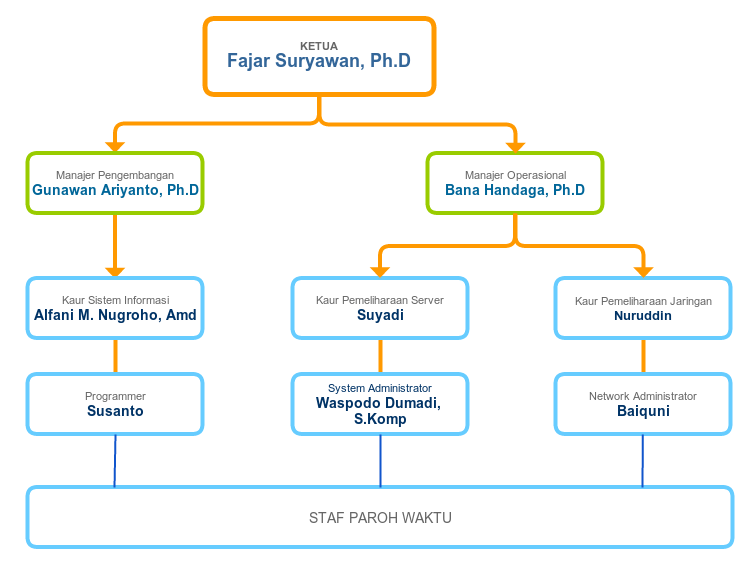
\includegraphics[width=1.0\textwidth]{pics/struktur.png}
\end{center}
\caption{Struktur Organisasi Unit IT UMS}
\end{figure}    


%-----------------------------------------------------------------------------%
\chapter{\babTiga}
%-----------------------------------------------------------------------------%
Penulis menggunakan \textit{framework} FAST (\textit{Framework for the Application of Systems Thinking}) dalam mengembangkan aplikasi ini. FAST mendefinisikan tahapan untuk mengidentifikasi dan mengevaluasi permasalahan-permasalahan, kesempatan-kesempatan, hambatan-hambatan yang terjadi, dan kebutuhan yang diharapkan sehingga dapat diusulkan perbaikan-perbaikan \cite{susanto2013}. 

\noindent
Fase-fase pengembangan menggunakan FAST diilustrasikan seperti \pic~\ref{fig:fast} \cite{whitten2007}.

\begin{figure}
	\centering
	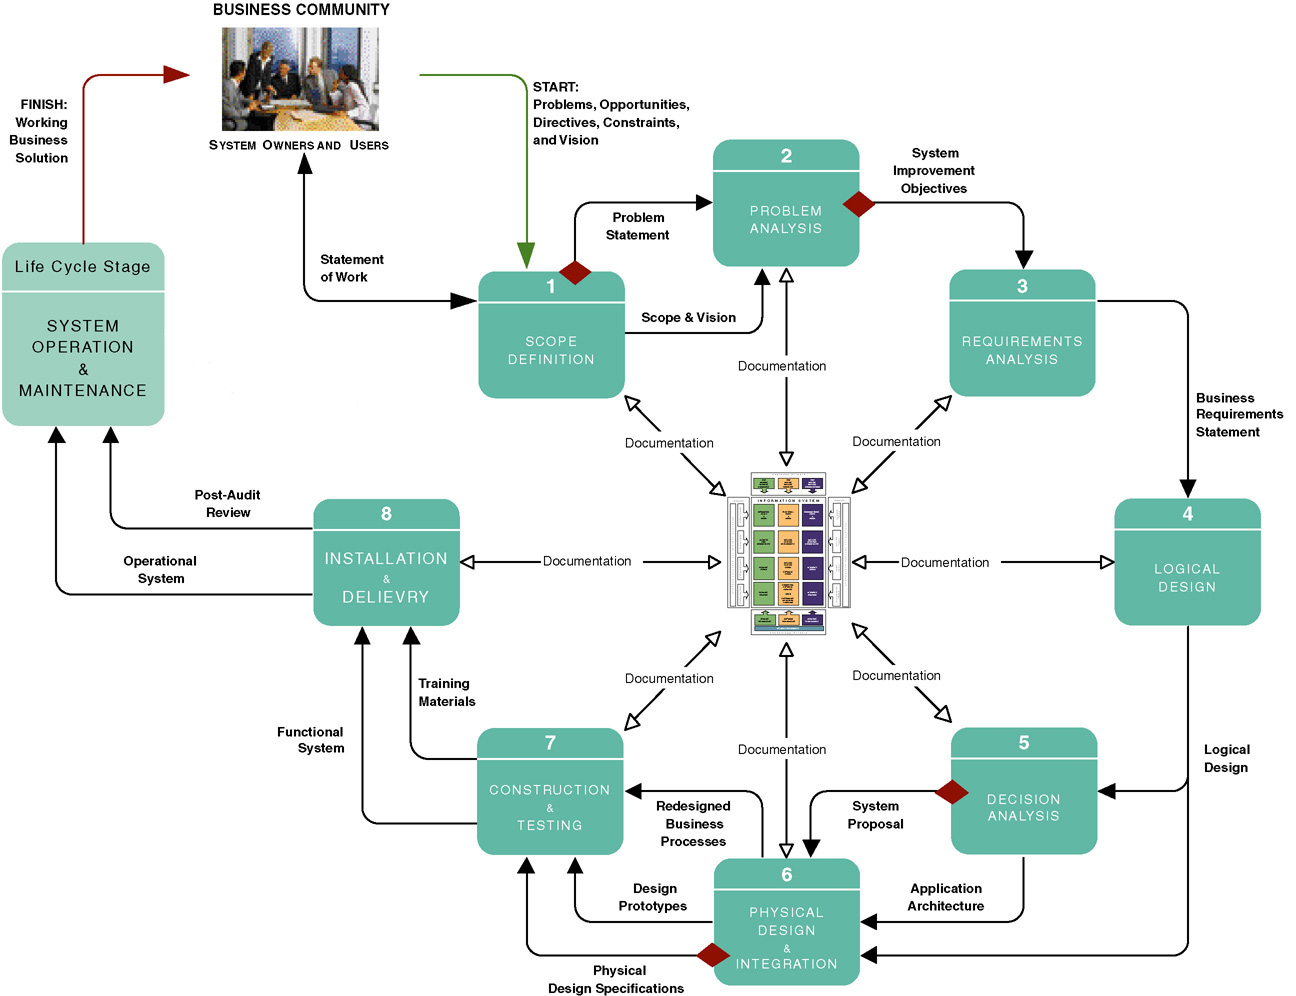
\includegraphics[width=1\textwidth]
		{pics/fastphase.jpg}
	\caption{Proses FAST framework}
	\label{fig:fast}
\end{figure}

\section{Definisi Lingkup}
Fase \f{scope definition} (definisi lingkup) ini digunakan untuk menetapkan  hal-hal sebagai berikut:

\begin{enumerate}[itemsep=-1ex]
\item Pernyataan masalah - pernyataan dan kategorisasi masalah, peluang dan arahan; juga dapat mencakup batasan dan visi awal untuk solusi, studi pendahuluan dan studi kelayakan.

\item Pembatas atau kendala - faktor pembatas yang mungkin membatasi solusi atau proses pemecahan masalah, termasuk di dalamnya besar anggaran, tenggat waktu, dan sumber daya manusia.

\item Pernyataan kerja - kontrak dengan manajemen dan komunitas pengguna untuk mengembangkan atau meningkatkan sistem informasi; mendefinisikan visi, ruang lingkup, batasan, kebutuhan pengguna, jadwal, dan anggaran.
\end{enumerate}

\section{Analisis Masalah}

Analisis masalah digunakan untuk mempelajari sistem yang ada  dan menganalisis temuan supaya tim proyek memiliki pemahaman yang menyeluruh tentang masalah yang memicu proyek.

Analis masalah sering mengungkap masalah baru dan menjawab pertanyaan yang paling penting, "Apakah manfaat dari pemecahan masalah ini melebihi biaya pembangunan sistem untuk memecahkan masalah ini?"

\section{Analisis Kebutuhan}

Analisis kebutuhan digunakan untuk menjawab pertanyaan-pertanyaan sebagai berikut: 
\begin{enumerate}[itemsep=-1ex]
\item Kemampuan apa yang harus disediakan sistem baru bagi penggunanya? 
\item Data apa yang harus ditangkap dan disimpan? 
\item Apa tingkat kinerja yang diharapkan? 
\item Apa prioritas dari berbagai kebutuhan?
\end{enumerate}

\section{Desain Logis}

Desain logis merupakan terjemahan dari kebutuhan pengguna bisnis ke dalam suatu model sistem yang menggambarkan hanya kebutuhan bisnis dan tidak ada desain teknis pelaksanaan kebutuhan tersebut. Desain ini meliputi desain konseptual dan desain penting. Model sistem adalah gambar sistem yang mewakili kenyataan atau realitas yang diinginkan. Model sistem memfasilitasi perbaikan komunikasi antara pengguna sistem, analis sistem, desainer sistem, dan pembangun sistem. 

Hal penting yang perlu diperhatikan juga pada tahap ini adalah pencegahan terjadinya \f{analysis paralysis}, sebuah istilah satir diciptakan untuk menggambarkan kondisi proyek umum di mana pemodelan sistem berlebihan secara dramatis memperlambat kemajuan menuju implementasi solusi sistem dimaksudkan.

\section{Analisis Keputusan}

Analisis keputusan digunakan untuk mengevaluasi kandidat sistem ditinjau berdasarkan:

\begin{enumerate}[itemsep=-1ex]
\item Kelayakan teknis: apakah solusi teknis praktis? Apakah staf kita memiliki keahlian teknis untuk merancang dan membangun solusi ini? 
\item Kelayakan operasional: apakah solusi yang memenuhi kebutuhan pengguna? Untuk tingkatan apa? Bagaimana solusi akan mengubah lingkungan kerja pengguna? Bagaimana pengguna mendapatkan manfaat dari solusi tersebut? 
\item Kelayakan ekonomi: apakah biaya solusi efektif? 
\item Jadwal kelayakan: dapatkah solusi dirancang dan dilaksanakan dalam waktu yang dapat diterima? 
\item Kelayakan Risiko: apa probabilitas keberhasilan implementasi menggunakan teknologi dan pendekatan?
\end{enumerate}

\section{Desain Fisik dan Integrasi}

Desain fisik merupakan terjemahan dari kebutuhan pengguna bisnis ke dalam suatu model sistem yang menggambarkan implementasi teknis kebutuhan bisnis pengguna. Sinonim umum termasuk desain teknis atau model implementasi. 

\noindent
Dua filosofi ekstrim desain fisik:
\begin{enumerate}[itemsep=-1ex]
\item \textit{Design by specification}: model sistem fisik dan spesifikasi rinci diproduksi sebagai rangkaian tertulis (atau yang dihasilkan komputer) cetak biru untuk konstruksi. 
\item \textit{Design by prototyping}: sistem tidak lengkap tetapi fungsi aplikasi dibangun dan disempurnakan berdasarkan masukan dari pengguna dan desainer lainnya.
\end{enumerate}

\section{Konstruksi dan Testing}
Fase pembangunan sistem yang meliputi: perangkat lunak, database, antarmuka sistem dan pengguna, perangkat keras, dan perangkat jaringan.

\section{Instalasi dan Penyerahan}
Fase instalasi dan penyerahan mencakup: instalasi sistem untuk dioperasikan yang sesungguhnya (\textit{production}), pelatihan pengguna, melengkapi dookumentasi, dan konversi data yang ada.
%-----------------------------------------------------------------------------%
\chapter{\babEmpat}
%-----------------------------------------------------------------------------%

\section{Definisi Lingkup}

\subsection{Pernyataan Masalah, Peluang dan Arahan}

Sebagaimana dipaparkan pada bab Pendahuluan, UMS telah memiliki sistem SSO dengan data \f{\gls{credential}} tersimpan dalam \GLS{ldap} dan dikelola dengan sebuah aplikasi tersendiri. Masalah yang muncul adalah bahwa data \GLS{ldap} sering tidak sinkron dengan data Sistem Informasi Kepegawaian dan Sistem Informasi Kemahasiswaan sebagai sumbernya. Di samping itu, terjadi dobel pekerjaan ketika menambah, mengubah dan menghapus data ke \GLS{ldap} dan server surel (\textit{Goole Apps}). 

\subsection{Pernyataan Tentang Solusi yang Diharapkan}
Aplikasi yang diusulkan memberikan lapisan antara yang menghubungan Sistem Informasi Kepegawaian dan Sistem Informasi Kemahasiswaan dengan \GLS{ldap} dan menghubungkan \GLS{ldap} dengan \textit{Google Apps}.

\begin{table}[ht]
  \centering
  \caption{Pernyataan Masalah dan Solusi}
  \renewcommand{\arraystretch}{1.5}% Spread rows out...
  \begin{tabular}
  {|>{}m{6.2cm}| 
    >{\centering}m{4cm}| 
    >{\centering\arraybackslash}m{2.50cm}|}
    \hline\hline
    \bo{Masalah, Peluang dan Arahan} & 
    \bo{Solusi yang Diajukan} & 
    \bo{Urutan Prioritas}\\
    \hline
    Data \GLS{ldap} sering tidak sinkron dengan data Sistem Informasi Kepegawaian dan Sistem Informasi Kemahasiswaan sebagai sumbernya.  & 
    Pengembangan aplikasi baru & 1 \\

   Terjadi dobel pekerjaan ketika menambah, mengubah dan menghapus data ke \GLS{ldap} dan server surel (\textit{Goole Apps}).  & 
    Pengembangan aplikasi baru & 2 \\

    \hline
  \end{tabular}
\end{table}


\newpage
\section{Analisis Masalah}

\begin{table}[ht]
\caption{Masalah, Peluang, Tujuan dan Pembatas}
\begin{tabular}{|p{3.75cm}|p{3cm}|p{3.50cm}|p{2cm}|}
\hline
\multicolumn{2}{|c|}{\bo{Analisis Sebab Akibat}} &
\multicolumn{2}{c|}{\bo{Tujuan Perbaikan Sistem}}\\
\hline
\centering \bo{Masalah/Peluang} & 
\centering \bo{Sebab Akibat} &
\centering \bo{Tujuan Sistem} &
\multicolumn{1}{c|}{\bo{Pembatas}}\\
\hline
\centering Data \GLS{ldap} sering tidak sinkron dengan data Sistem Informasi Kepegawaian dan Sistem Informasi Kemahasiswaan sebagai sumbernya. &
\centering Terjadi duplikasi data dan data \GLS{ldap} tidak tervalidasi. &
\centering Dibuat aplikasi web service yang memungkinkan untuk menghidari duplikasi data dan memvalidasinya. & 
{Aplikasi harus aman.}\\
\hline
\centering Terjadi dobel pekerjaan ketika menambah, mengubah dan menghapus data ke \GLS{ldap} dan server surel (\textit{Goole Apps}). &
\centering Pekerjaan tidak efisien. &
\centering Dibuat aplikasi web service yang memungkinkan sinkronisasi \GLS{ldap} dengan \textit{Google Apps} secara otomatis. &
{Aplikasi harus aman.} \\
\hline
\end{tabular}
\end{table}

\newpage
\section{Analisis Kebutuhan}

\begin{table}[ht]
  \caption{Daftar Kebutuhan}
  \renewcommand{\arraystretch}{1.5}% Spread rows out...
  \begin{tabular}
  {|>{}m{10.75cm}| 
    >{\centering\arraybackslash}m{2.5cm}|}
    \hline\hline
    \bo{Kebutuhan} & 
    \bo{Klasifikasi}\\
    \hline
    Sistem harus mengijinkan aplikasi ter-authentikasi menelusur data pengguna. &
    Fungsional\\
    \hline
    Sistem harus mengijinkan aplikasi ter-authentikasi menambah, mengubah dan menghapus data pengguna. &
    Fungsional\\
    \hline
    Sistem harus mengijinkan aplikasi ter-authentikasi menambah, mengubah dan menghapus data \gls{surel} pengguna. &
    Fungsional\\
    \hline
    Sistem harus mengijinkan aplikasi ter-authentikasi melakukan sinkronisasi data pengguna ke \textit{Google Apps}. &
    Fungsional\\
    \hline
    Sistem harus mengijinkan aplikasi ter-authentikasi mengubah password \textit{Google Apps}. &
    Fungsional\\
    \hline
    Sistem harus mengijinkan aplikasi ter-authentikasi menampilkan \gls{surel} alias pengguna \textit{Google Apps}. &
    Fungsional\\
    \hline
    Sistem harus mengijinkan aplikasi ter-authentikasi menampilkan dan mengubah alamat pengiriman \gls{surel} pengguna \textit{Google Apps}. &
    Fungsional\\
    \hline
    Sistem harus mengijinkan aplikasi ter-authentikasi mendelegasikan akun \gls{surel} pengguna \textit{Google Apps}. &
    Fungsional\\
    \hline
    Sistem yang dibangun adalah \textit{web service} menggunakan bahasa pemrograman Python&
    Non fungsional\\
    \hline
  \end{tabular}
\end{table}

\newpage
\section{Desain Logis}

\subsection{Use-case}

\singlespacing
\begin{table}[H]
\caption{Daftar \textit{Use-case}}
\renewcommand{\arraystretch}{1.5}% Spread rows out...
\begin{tabular}
{|>{\centering}m{4cm}|
   >{\centering}m{7.25cm}| 
   >{\centering\arraybackslash}m{2cm}|}
\hline\hline
\bo{Nama Use-case} & \bo{Deskripsi Use-case} & \bo{Aktor}\\
\hline
Menelusur Data Pengguna &
Use-case yang mendeskripsikan proses penelusuran data \GLS{ldap} &
\acrshort{api} Client\\
\hline
Menambah, Mengubah dan Menghapus Data Pengguna &
Use Case yang mendeskripsikan proses menambah, mengubah dan menghapus data pengguna di \GLS{ldap} &
\acrshort{api} Client\\
\hline
Menampilkan, Menambah dan Menghapus Email Pengguna &
Use Case yang mendeskripsikan proses menampilkan, menambah dan menghapus \gls{surel} pengguna di \GLS{ldap} &
\acrshort{api} Client\\
\hline
Menampilkan, Menambah dan Menghapus Jabatan Pengguna &
Use Case yang mendeskripsikan proses menampilkan, menambah dan menghapus jabatan pengguna di \GLS{ldap} &
\acrshort{api} Client\\
\hline
Sinkronisasi Data ke \textit{Google Apps} &
Use Case yang mendeskripsikan proses sinkronisasi data ke \textit{Google Apps} &
\acrshort{api} Client\\
\hline
Mengubah Password \textit{Google Apps} &
Use Case yang mendeskripsikan proses mengubah password pengguna di \textit{Google Apps} &
\acrshort{api} Client\\
\hline
Menampilkan Alias Email \textit{Google Apps} &
Use Case yang mendeskripsikan proses menampilkan alias \gls{surel} pengguna di \textit{Google Apps} &
\acrshort{api} Client\\
\hline
Menampilkan dan Menambah Alamat Pengiriman Email \textit{Google Apps} &
Use Case yang mendeskripsikan proses menampilkan dan menambah alamat pengiriman \gls{surel} pengguna di \textit{Google Apps} &
\acrshort{api} Client\\
\hline
Mengelola Delegasi Email \textit{Google Apps}&
Use Case yang mendeskripsikan proses pendelegasian \gls{surel} pengguna di \textit{Google Apps} &
\acrshort{api} Client\\
\hline
\end{tabular}
\end{table}
\doublespacing

\subsection{Daftar Entitas}

\textbf{Atribut LDAP yang digunakan} \cite{biondo2001}:\\
uid: user id unik/nama login\\
givenName: nama depan\\
sn: nama belakang\\
cn: nama lengkap\\
userPassword: password\\
postalAddress: alamat\\
l: kota\\
st: propinsi\\
postalCode: kode pos\\
mail: alamat surel\\
telephoneNumber: telpon rumah\\
mobile: nomor hp\\
employeeNumber: NIK/NIP\\
employeeType: jenis karyawan/mahasiswa\\
departmentNumber: nomor unit/fakultas\\
ou: nama unit/fakultas\\

\subsection{Model Proses}

\begin{figure}
	\centering
	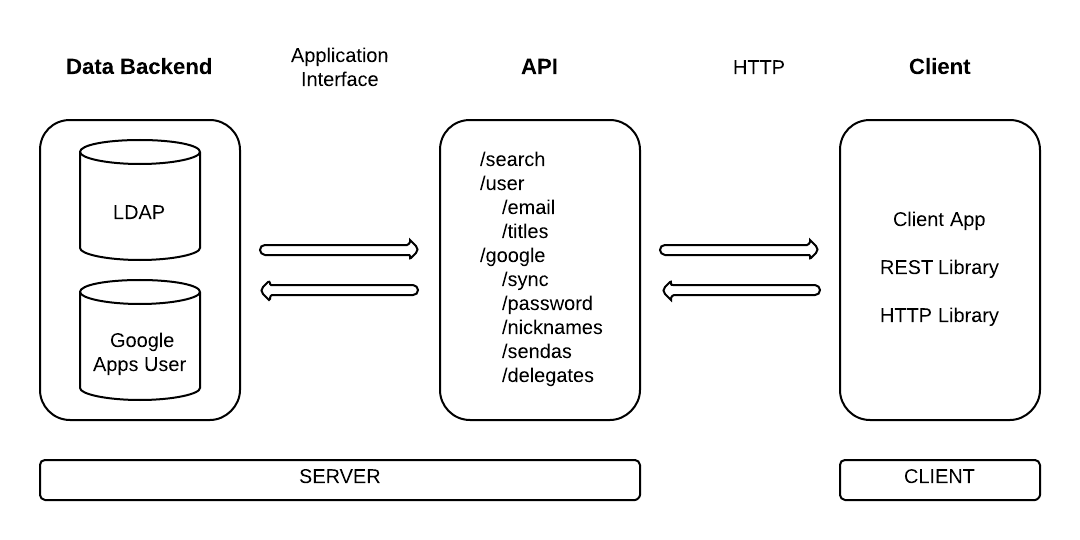
\includegraphics[width=1\textwidth]
		{pics/processmodel.png}
	\caption{Model Proses}
	\label{fig:model}
\end{figure}

\section{Desain Fisik}

Aplikasi yang dibangun menggunakan authentikasi \textit{Basic Authentication} yang merupakan kombinasi \textit{username} dan \textit{password}. \textit{Request} dan \textit{Response} hanya menggunakan format \textit{JSON}.

\subsection{Menelusur Data Pengguna}

POST https://accounts.ums.ac.id/search

\noindent
\textit{JSON Request:}
\begin{lstlisting}
{
    "filter": "uid=ya931"
}
\end{lstlisting}

\noindent
\textit{JSON Response:}
\begin{lstlisting}
[
    [
        "uid=ya931,ou=Employee,ou=People,dc=ums,dc=ac,dc=id",
        {
            "uid": ["ya931"],
            "givenName": ["Suyadi"],
            "sn": ["Abufarros"],
            "cn": ["Suyadi Abufarros"],
            "postalAddress": ["Purbayan Baki"],
            "l": ["Sukoharjo"],
            "st": ["Jateng"],
            "c": ["Indonesia"],
            "postalCode": ["57102"],
            "mail": ["suyadi@ums.ac.id", "abufarros@gmail.com"],
            "telephoneNumber": ["0271222222"],
            "mobile": ["081234556"],
            "employeeNumber": ["931"],
            "employeeType": ["Karyawan Tetap"],
            "departmentNumber": ["345"],
            "ou": [ "UIT"],
            "title": ["STAF"]
        }
    ],
]
\end{lstlisting}

\subsection{Menambah Data Pengguna}

POST https://accounts.ums.ac.id/users

\noindent
\textit{JSON Request:}
\begin{lstlisting}
{
    "userType": "EMPLOYEE",
    "uniID": "abc123",
    "firstName": "Muhammad",
    "lastName": "Surono",
    "userPassword": "qwerty",
    "postalAddress": "Pabelan",
    "city": "Solo",
    "state": "Jateng",
    "postalCode": "57102",
    "mail": "abc123@gmail.com",
    "telephoneNumber": "0271222222",
    "mobile": "081234556",
    "employeeNumber": "876",
    "employeeType": "Dosen",
    "departmentNumber": "345",
    "ou": "Teknik Informatika"
}
\end{lstlisting}

\noindent
\textit{Text Response:}\\
- \textbf{Ok}: berhasil menambahkan data\\
-  \textbf{Not ok}: gagal menambahkan data

\subsection{Mengubah Data Pengguna}

PUT https://accounts.ums.ac.id/users

\noindent
\textit{JSON Request:}
\begin{lstlisting}
{
    "userType": "EMPLOYEE",
    "uniID": "abc123",
    "firstName": "Muhammad",
    "lastName": "Surono",
    "userPassword": "qwerty",
    "postalAddress": "Pabelan",
    "city": "Solo",
    "state": "Jateng",
    "postalCode": "57102",
    "mail": "abc123@gmail.com",
    "telephoneNumber": "0271222222",
    "mobile": "081234556",
    "employeeNumber": "876",
    "employeeType": "Dosen",
    "departmentNumber": "345",
    "ou": "Teknik Informatika"
}
\end{lstlisting}

\noindent
\textit{Text Response:}\\
- \textbf{Ok}: berhasil menambahkan data\\
-  \textbf{Not ok}: gagal menambahkan data

\subsection{Menghapus Data Pengguna}

DELETE https://accounts.ums.ac.id/users

\noindent
\textit{JSON Request:}
\begin{lstlisting}
{
    "uniID": "abc123"
}
\end{lstlisting}

\noindent
\textit{Text Response:}\\
- \textbf{Ok}: berhasil menambahkan data\\
-  \textbf{Not ok}: gagal menambahkan data


\subsection{Menampilkan Email Pengguna}

POST https://accounts.ums.ac.id/user/email

\noindent
\textit{JSON Request:}
\begin{lstlisting}
{
    "uniID": "ya931"
}
\end{lstlisting}

\noindent
\textit{JSON Response:}
\begin{lstlisting}
[
    "Suyadi@ums.ac.id",
    "Suyadi.Abufarros@ums.ac.id"
]
\end{lstlisting}

\subsection{Menambah Email Pengguna}

PUT https://accounts.ums.ac.id/user/email

\noindent
\textit{JSON Request:}
\begin{lstlisting}
{
    "uniID": "ya931",
    "email": "suyadi@ums.ac.id"
}
\end{lstlisting}

\noindent
\textit{Text Response:}\\
- \textbf{Ok}: berhasil menambahkan data\\
-  \textbf{Not ok}: gagal menambahkan data

\subsection{Menghapus Email Pengguna}

DELETE https://accounts.ums.ac.id/user/email

\noindent
\textit{JSON Request:}
\begin{lstlisting}
{
    "uniID": "ya931",
    "email": "suyadi@ums.ac.id"
}
\end{lstlisting}

\noindent
\textit{Text Response:}\\
- \textbf{Ok}: berhasil menambahkan data\\
-  \textbf{Not ok}: gagal menambahkan data

\subsection{Menampilkan Jabatan Pengguna}

POST https://accounts.ums.ac.id/user/titles

\noindent
\textit{JSON Request:}
\begin{lstlisting}
{
    "uniID": "ya931"
}
\end{lstlisting}

\noindent
\textit{JSON Response:}
\begin{lstlisting}
[
    "CNF",
    "Admin"
]
\end{lstlisting}

\subsection{Menambah Jabatan Pengguna}

PUT https://accounts.ums.ac.id/user/titles

\noindent
\textit{JSON Request:}
\begin{lstlisting}
{
    "uniID": "ya931",
    "title": "Admin"
}
\end{lstlisting}

\noindent
\textit{Text Response:}\\
- \textbf{Ok}: berhasil menambahkan data\\
-  \textbf{Not ok}: gagal menambahkan data

\subsection{Menghapus Jabatan Pengguna}

DELETE https://accounts.ums.ac.id/user/titles

\noindent
\textit{JSON Request:}
\begin{lstlisting}
{
    "uniID": "ya931",
    "title": "Admin"
}
\end{lstlisting}

\noindent
\textit{Text Response:}\\
- \textbf{Ok}: berhasil menambahkan data\\
-  \textbf{Not ok}: gagal menambahkan data

\subsection{Sinkronisasi Data ke \textit{Google Apps}}

POST https://accounts.ums.ac.id/google/sync

\noindent
\textit{JSON Request:}
\begin{lstlisting}
{
    "uniID": "ya931"
}
\end{lstlisting}

\noindent
\textit{Text Response:}\\
- \textbf{Ok}: berhasil menambahkan data\\
-  \textbf{Not ok}: gagal menambahkan data

\subsection{Mengubah Password \textit{Google Apps}}

POST https://accounts.ums.ac.id/google/password

\noindent
\textit{JSON Request:}
\begin{lstlisting}
{
    "uniID": "ya931",
    "password": "mypassword"
}
\end{lstlisting}

\noindent
\textit{Text Response:}\\
- \textbf{Ok}: berhasil menambahkan data\\
-  \textbf{Not ok}: gagal menambahkan data

\subsection{Menampilkan Alias Email \textit{Google Apps}}

POST https://accounts.ums.ac.id/google/nicknames

\noindent
\textit{JSON Request:}
\begin{lstlisting}
{
    "uniID": "ya931"
}
\end{lstlisting}

\noindent
\textit{JSON Response:}
\begin{lstlisting}
[
    "suyadi",
    "suyadi.abufarros"
]
\end{lstlisting}

\subsection{Menampilkan Alamat Pengiriman Email \textit{Google Apps}}

POST https://accounts.ums.ac.id/google/sendas

\noindent
\textit{JSON Request:}
\begin{lstlisting}
{
    "uniID": "ya931",
}
\end{lstlisting}

\noindent
\textit{JSON Response:}
\begin{lstlisting}
[
    "suyadi@ums.ac.id",
    "suyadi.abufarros@ums.ac.id"
]
\end{lstlisting}

\subsection{Menambah Alamat Pengiriman Email \textit{Google Apps}}

PUT https://accounts.ums.ac.id/google/sendas

\noindent
\textit{JSON Request:}
\begin{lstlisting}
{
    "uniID": "ya931",
    "address": "suyadi@ums.ac.id"
}
\end{lstlisting}

\noindent
\textit{Text Response:}\\
- \textbf{Ok}: berhasil menambahkan data\\
-  \textbf{Not ok}: gagal menambahkan data

\subsection{Menampilkan Delegasi Email \textit{Google Apps}}

POST https://accounts.ums.ac.id/google/delegates

\noindent
\textit{JSON Request:}
\begin{lstlisting}
{
    "uniID": "ithelpdesk"
}
\end{lstlisting}

\noindent
\textit{JSON Response:}
\begin{lstlisting}
[
    "ya123@ums.ac.id",
    "wd123@ums.ac.id"
]
\end{lstlisting}

\subsection{Menambah Delegasi Email \textit{Google Apps}}

PUT https://accounts.ums.ac.id/google/delegates

\noindent
\textit{JSON Request:}
\begin{lstlisting}
{
    "uniID": "ithelpdesk",
    "nickname": "ya123@ums.ac.id"
}
\end{lstlisting}

\noindent
\textit{Text Response:}\\
- \textbf{Ok}: berhasil menambahkan data\\
-  \textbf{Not ok}: gagal menambahkan data

\subsection{Menghapus Delegasi Email \textit{Google Apps}}

DELETE https://accounts.ums.ac.id/google/nicknames

\noindent
\textit{JSON Request:}
\begin{lstlisting}
{
    "uniID": "ithelpdesk",
    "nickname": "ya123@ums.ac.id"
}
\end{lstlisting}

\noindent
\textit{Text Response:}\\
- \textbf{Ok}: berhasil menambahkan data\\
-  \textbf{Not ok}: gagal menambahkan data

\section{Konstruksi dan Testing}

Penulis menggunakan \textit{Flask Framework} dalam mengembangkan aplikasi ini. \textit{Flask} adalah sebuah \textit{framework} mikro untuk mengembangkan aplikasi web berbahasa \textit{Python}. "Mikro" bukan berarti aplikasi web yang dibuat hanya terdiri dari sebuah file, walaupun memungkinkan, juga bukan berarti memiliki fungsionalitas terbatas, tetapi lebih ditekankan pada kesedarhanaan  dan \textit{extensible}.

Untuk mengembangkan aplikasi berbasis \textit{Flask} tidak memerlukan spesifikasi perangkat yang tinggi, tetapi butuh koneksi internet, karena data \textit{Google Apps} tersimpan di server \textit{Google}. Secara rinci, kebutuhan pengembangan aplikasi ini sebagai berikut:

\begin{enumerate}[itemsep=-1ex]
\item Laptop dengan sistem operasi Windows, Linux atau sistem operasi lain yang kompatibel dengan \textit{Python}.
\item Bahasa pemrograman \textit{Python} dan \textit{Python Setuptools}.
\item Beberapa paket \textit{Python} yang dibutuhkan: \textit{Flask, Python-LDAP, Gdata, dll.}
\end{enumerate}

%\lstinputlisting[language=Python]{code/simple-client/simple.py}

\section{Instalasi}

Ada beberapa cara untuk menginstall aplikasi ke server produksi yang salah satunya menggunakan \textit{Gunicorn} dan \textit{Nginx} pada \textit{Linux Debian}. \textit{Gunicorn (Green Unicorn)} adalah \textit{Web Server Gateway Interface (WSGI)}. \textit{Nginx} adalah web server yang difungsikan sebagai \textit{proxy}. Menurut Benoit Chesneau, sangat direkomendasikan \textit{Gunicorn} digunakan bersama \textit{proxy} server \cite{benoit2012}.
%---------------------------------------------------------------
\chapter{\kesimpulan}
%---------------------------------------------------------------

%---------------------------------------------------------------
\section{Simpulan}
%---------------------------------------------------------------


%---------------------------------------------------------------
\section{Saran}
%---------------------------------------------------------------


%
% Daftar Pustaka
%
% Daftar Pustaka 
% 

% 
% Tambahkan pustaka yang digunakan setelah perintah berikut. 
% 
\begin{thebibliography}{4}

\bibitem{luthfi2012}
{Abdurrahman, Luthfi. (2012). 
\f{Implementasi Sistem Single Sign-On Menggunakan OpenAM dengan Otentikasi Kerberos dan OpenLDAP} (online).
url: \url{http://repository.usu.ac.id/handle/123456789/31207.}}

\bibitem{benoit2012}
{Benoit Chesneau. (2012).
\textit{Deploying Gunicorn} (online).
\url{http://gunicorn-docs.readthedocs.org/en/latest/deploy.html}.
diakses: 21 Mei 2014.}

\bibitem{biondo2001}
{Biondo, Giuseppe Lo. (2001). 
\f{LDAP Implementation HOWTO} (online).
\url{http://www.tldp.org/HOWTO/archived/LDAP-Implementation-HOWTO/schemas.html}.
diakses: 13 Mei 2014.}

\bibitem{nugroho2009}
{Nugroho, Lukito Edi. (2009). 
\f{Pemanfaatan Teknologi Informasi di Perguruan Tinggi}.
Yogyakarta, Prajnya Media.}

\bibitem{susanto2013}
{Susanto, Hari. (2013). \f{Sekilas FAST (Framework for the Applications of System Technology)}. online: \url{http://hari-cio-8a.blog.ugm.ac.id/2013/04/04/sekilas-fast-framework-for-the-applications-of-system-technology/}, diakses: 11 Mei 2014.}

\bibitem{whitten2007}
{Whitten, Jeffrey L. and Lonnie D. Bentley. (2007).
\f{Systems analysis and design methods.--7th ed.} McGraw-Hill Irwin.}

\end{thebibliography}



%
% Lampiran 
%
%\begin{appendix}
%	%
% @author  Andreas Febrian
% @version 1.00 
% 
% Hanya sebuah pembatas bertuliskan LAMPIRAN ditengah halaman. 
% 

\begin{titlepage}
	\centering 
	\vspace*{6cm}
	\noindent \Huge{LAMPIRAN}
	\addChapter{LAMPIRAN}
\end{titlepage}
%	\setcounter{page}{2}
%	%-----------------------------------------------------------------------------%
\addChapter{Lampiran 1}
\chapter*{Lampiran 1}
%-----------------------------------------------------------------------------%
%\end{appendix}

\end{document}